%*******************************************************************************
%****************************** Second Chapter *********************************
%*******************************************************************************

\chapter{Related Work}
\label{chapter_related}

\section{Related Work Overview}
\label{section_related}

\ifpdf
    \graphicspath{{Chapter2/Figs/Raster/}{Chapter2/Figs/PDF/}{Chapter2/Figs/}}
\else
    \graphicspath{{Chapter2/Figs/Vector/}{Chapter2/Figs/}}
\fi

Since there are many different related work areas that all have their relevance to this thesis, this chapter is divided into different sections dealing with each of them in turn. Section \ref{subsec_patternMining} gives an overview on classical pattern mining and frequent itemset mining approaches. Section \ref{subsec_regression} continues with an outline of the state of the art classification and regression approaches after which section \ref{subsec_prediction} will take a closer look on time series prediction with a focus on financial data and stock market forecasting.
Section \ref{subsec_dataStreamProcessing} then introduces related work in the very broad research area of processing and mining data streams. Afterwards section \ref{subsec_eventProcessing} presents the research area of general event processing with a focus on the mining of complex events and episodes. Finally section \ref{subsec_semanticWeb} finishes with an overview over the most relevant work (with respect to this thesis) in the research area of the semantic web.

\subsection{Pattern Mining}
\label{subsec_patternMining}
Of all the fields related to this thesis basic pattern mining is arguably the most well researched and widely used related research area. First to mention are of course the standard pattern mining algorithms for frequent itemsets \cite{han2007frequent}. The authors of this paper nicely summarize different approaches, which either use candidate generation and the apriori-principle or pattern growth strategies. Problematic with the original Apriori-Algorithm is of course that while the apriori-principle helps to prune the candidate generation, its runtime can still be exponential. On top of that it requires multiple passes over the database, which is something that can be impossible given large data streams. These general pattern mining algorithms have of course already been modified or improved for more specific purposes. For example event data logs have been used to build predictive models that search for patterns that predict critical events in the log file \cite{chen2014pattern}. \newline
A rather large subfield of pattern mining is the field of (business) process mining. This particular domain usually evaluates log-files of (business) applications that log sequences of events. These logs can be mined to satisfy many different information needs, for example clustering \cite{vaarandi2015logcluster} or process models \cite{priyadharshini2016analysis}.
Another approach in the field of business logs and process mining is outlier and anomaly detection \cite{sureka2015kernel}. The authors use the length of the longest common subsequence between event sequences as a distance measure to find unusual patterns of events. This field of interest is especially interesting since there are a lot of business applications, some of which use legacy software, whose behaviour is at times unclear or error-prone. Mining underlying business models or unusual behavior can help identify errors. \newline
A subfield of pattern mining that is especially relevant for this thesis is sequential pattern mining. Comprehensive overviews are given by Slimani et al. \cite{slimani2013sequential} as well as Zhao at al. \cite{zhao2003sequential}.

\subsection{Classification and Regression}
\label{subsec_regression}

Classification and regression are the main applications of supervised learning. They are very similar and closely interlinked to each other. Classification aims to assign new, unseen objects to a class based on a model that was created from training data. Class labels are categorical. Regression is similar, but instead of assigning categorical class labels to new data points it is now the goal to generate a numerical (real) value that is close to the actual value. 
A comprehensive overview over most classification approaches was comprised by Kotsiantis et. al. \cite{kotsiantis2007supervised}. The authors distinguish between different types of classifiers:
\begin{itemize}
	\item logical classifiers such as Decision Trees and rule based algorithms
	\item preceptron based classifiers, such as the single layered perceptron or artificial neural networks
	\item statistical classifiers, such as naive bayes or bayesian networks
	\item instance based classifiers, such as k nearest neighbor
	\item maximum margin classifiers, such as support vector machines
\end{itemize}
It is notable that the authors do not mention ensemble learners \cite{dietterich2000ensemble}, which combine several classifiers and classify new examples by letting each classifier vote. Arguably the most notable ensemble learning technique is the random forest \cite{liaw2002classification}.
It is important to keep in mind that most classification approaches can also be tweaked to do regression, a random forest for instance can either be used to estimate a (binary) class label (classification) or a numerical value (regression).
Classification and regression have also been attempted by using pattern mining and association rule generation \cite{ma1998integrating}. Instead of mining all association rules the authors focus on finding so called class association rules. An especially relevant application of rule based regression was the usage of classification rules using minimal rule generation for the prediction of equity returns \cite{apte1994predicting}. The authors modify a classification rule generation technique called R-MINI to be able to do regression. They evaluate their approach on historical stock market data from the S\&P 500 data-set (data is aggregated to monthly values). 
%While both of these pieces of work are interesting and extremely relevant to the problem tackled by this thesis it is important to note that they were both done in 1998 and 1994 respectively, so it is expected that the state of the art has changed since then.

\subsection{Prediction and Financial Time Series Forecasting}
\label{subsec_prediction}
Similar to regression and classification, but not quite the same is prediction. Prediction (sometimes also called forecasting) introduces a new dimension, which is time. The task in prediction is to build a model that if given data points on a timeline will predict which data point will show up next.
Due to its dependency on time, prediction plays a large role when mining time series data. Arguably the most popular models for time series prediction are artificial neural networks which are used by multiple authors with differnt variations and application domains \cite{connor1994recurrent} \cite{martinetz1993neural} \cite{frank2001time}. Of particular interest for this thesis are of course prediction approaches that were used in the same domain, namely stock market or financial time series prediction. Naturally this has been looked into. Gestel at. al. used support vector machines to predict the closing values of stock market indices \cite{van2001financial}.% (TODO: Talk/Read more about this paper, the bayesian networks, that are used too) 
Another, more recent approach used an artificial neural network with an improved learning algorithm (by integrating improved bacterial chemotaxis optimization into the back propagation of the neural network) to successfully predict the Standard’s \& Poor’s 500 index (changes were aggregated to daily values).
Another different approach is to use grey system models to predict time series \citep{kayacan2010grey}, in this specific case the authors predict the daily foreign currency exchange rate of euro to dollar. A comprehensive comparison of different models for predicting the S\&P CNX NIFTY index was carried out by kumar et. al. \citep{kumar2006forecasting}. The best performing model in their study is the support vector machine, closely followed by a random forest. This is interesting, since random forests have not received as much attention for time series prediction as for example artificial neural networks. Of course no general conclusions can be drawn from the performance of these models for one index. An very detailed overview over a lot of work in the area can be found in the literature study done by Atsalakis et al. \cite{atsalakis2009surveying} although the focus seems to be on papers that use neural networks or support vector machines.
The attentive reader will have noticed that most of the previously named examples focus on predicting stock indices, a.k.a the general direction of the market. Predicting individual stock values has been looked at less, but there is of source some previous work to be considered. For example mahfoud et. al. compare genetic algorithms to neural networks for the prediction of individual stocks \cite{mahfoud1996financial}.

\subsection{Data Stream Processing}
\label{subsec_dataStreamProcessing}
Many research areas in classical data mining are also of interest when processing streams. As already mentioned in the introduction however, data streams impose severe restrictions on the algorithms, such them having to use only one pass over the data and that they must be incremental. Almost no data mining algorithms for the classical scenario in which the underlying data is a static database or even a data-set that fits into main memory have these properties. Thus the algorithms need to be modified and often approximations have to be made. A comprehensive basic overview over the application of different data mining tasks and how they can be applied to streams was comprised by Gaber et. al. \cite{gaber2005mining}. \newline
As already mentioned many data mining algorithms for data streams make compromises of some sort or employ appoximations. Especially in the area of pattern mining there are quite a few approaches that use approximations or focus on the most recent data. Gianella et. al. have for example developed an algorithm to incrementally maintain approximately frequent itemsets for the most recent time windows using tilted time window frames \cite{giannella2003mining}. Approaches to mine frequent items without tilting the time windows exist as well, such as the sticky sampling or the lossy counting algorithm \cite{manku2002approximate}. These algorithms can be generalized to mine frequent itemsets, too. If this is done however pruning the candidates may become an issue if the main memory is small (the number of candidates to maintain may be too large). \newline
A paper also related to regression and time series forecasting was published by Papadimitriou et. al. \cite{papadimitriou2003adaptive}. The authors tackle the problem of cyclic time series mining, as well as time series prediction of numerical values in potentially infinite data streams. \newline
The rise in popularity of mining data streams also pushes research areas like distributed data mining, in which parallelized versions of data mining algorithms are researched. Large data streams and distributed systems often go hand in hand, which creates the need for distributed algorithms. Such solutions have been researched for example for frequent pattern mining \cite{lin2015fast}, association rule mining \cite{ashrafi2004odam}, clustering \cite{januzaj2004dbdc} and classification (in this case a distributed boosting algorithm) \cite{lazarevic2001distributed}. \newline
A slightly different direction to data stream processing is querying data streams. Some contributing data scientists have thus approached streams in a similar manner as relational databases \cite{motwani2003query}. The authors present their progress at building a general purpose Data Stream Management System (DSMS) prototype, as a pendant to the traditional Database Management Systems (DBMS). They suggest the usage of an extension of SQL as a stream query language to allow for continuous queries and discuss approximation techniques. 

\subsection{Complex Event Processing and Episode Mining}
\label{subsec_eventProcessing}
Before talking about the state of the art in complex event processing it is first important to clarify the term \textit{"event"} which is a is very broad term that is used in many different areas of science. Even when restricted to computer science there may be different definitions with subtle differences. As already explained in the introduction this thesis will focus on events as defined by the glossary of the event processing society \cite{luckham2011epts}.
When talking about processing complex events there is an important difference between two cases:

\begin{itemize}
	\item The patterns of interest are known before looking at the data. This is called complex event detection.
	\item There is no prior knowledge about which patterns might be interesting, they need to be discovered while looking at the data. This is called complex event discovery or complex event mining (which basically means that data mining methods need to be employed)
\end{itemize}

Complex event detection usually revolves around specification and query languages for complex events \cite{eckert2009complex}. Quite a few different specification and query languages have been developed, such as SNOOP \cite{chakravarthy1994snoop} or the SASE event processing language \cite{wu2006high}. \newline
Discovering interesting complex events of arbitrary structure in data streams is a very challenging task, thus most work focuses on specific types of complex events. A popular example is mining frequent sequences of events (basically complex events that only use the sequence operator) \cite{bettini1998mining} \cite{hasan2015probabilistic}. \newline
This thesis deals with a more expressive type of complex events: Episodes. Originally episodes were researched without any relation to event processing \cite{mannila1995discovering}. 
Episodes have roughly been categorized as serial, parrallel or composite and there are different mining methods proposed for each of these \cite{mannila1995discovering} \cite{zhou2010mining}. The connection between episodes and hidden markov models was also explored in a PHD thesis by Laxman \cite{laxman2006discovering}.
Evaluating episode mining algorithms on real-life datasets is often difficult due to a lack of knowledge about the ground truth. Thus, generation of realistic, synthetic datasets has been looked into as well \cite{zimmermann2012generating}.

\subsection{Semantic Web}
\label{subsec_semanticWeb}
TODO


\section{Basic Definitions and Terminology}
This section introduces relevant definitions and terminology that was introduced in previous work and will be used in this thesis.

\subsection{Event Processing Terminology}
Most of the basic event terminology in this subsection is taken from the event processing glossary created by the Event Processing Technical Society \cite{luckham2011epts}. Note that some of the definitions may be slightly altered or simplified. This is due to the fact that the event processing technical society uses these terms for a very general description of event processing and event processing architectures and thus some original definitions are more complex than what is needed in this thesis. The definitions given here aim to establish a clear terminology for this thesis.

\begin{mydef}
\textbf{Event} An event is either something that is happening in the real world or in the context of computer science an object that represents a real world event and records its properties. The latter can also be referred to as an event object or an event tuple. Note that the term is overloaded, but the context usually gives a clear indication of what is meant.
\end{mydef}

\begin{mydef}
\textbf{Simple Event} A simple event is an event that is not viewed as summarizing, representing, or denoting a set of other events. Sometimes also referred to as a basic events.
\end{mydef}

These two definitions can sometimes cause confusion. It is important to note that the term event is the most general term, since it can refer to any kind of event, be it simple, derived or complex (TODO: better, see below for definitions, or move this note). A simple event however is the most basic form of an event and often the ingredient for the creation of more complex events:
Given a simple events it is possible to derive events from those or the absence of those. For example the absence measurement events of sensor $A$ could be used to derive the event of the sensor $A$ becoming defect. These events are called derived events:

\begin{mydef}
\textbf{Derived Event} A derived Event or synthesized event is an event that is generated according to some method or based on some reasoning process.
\end{mydef}

It is also possible to combine multiple simple events to form what we refer to as complex events:

\begin{mydef}
\textbf{Complex Event} A complex event is a derived event that is created by combining other events. The events can be combined by using certain operators, for example disjunction, conjunction or sequence. An example would be $(A \land B) \rightarrow C$ (event A and B in any order followed by event C).
\end{mydef}

This is a very broad definition of complex events. The choice of allowed operators strongly impacts the expressiveness of complex events. A specific kind of complex events are episodes (see TODO: reference), which will be the main focus of this thesis.
The next notion that needs to be considered is that each individual event normally belongs to a certain class of events, which we refer to as the event type:

\begin{mydef}
textbf{Event type} The event type, sometimes also referred to as event class, event definition, or event schema is a label that identifies events as members of an event class.
\end{mydef}

Another important term that was not defined in the event processing glossary, but is very relevant to the topic at hand is the notion of a type alphabet:

\begin{mydef}
textbf{Type Alphabet} The event alphabet is the set of all possible event types that can occur in the observed system.
\end{mydef}

Event alphabets are often implicitly defined when mining frequent itemsets, patterns or episodes (see definition below).
So far we have looked at events without considering the scenario we are most interested in which are event streams. To do so we need the notion of timestamps:

\begin{mydef}
\textbf{Timestamp} A time value of an event indicating its creation or arrival time.
\end{mydef}

Given that we can define an event stream:

\begin{mydef}
\textbf{Event Stream} An event stream is an ordered sequence of events, usually ordered by the event timings.
\end{mydef}

Note that this rather broad definition of an event stream does not assume anything about the kind of event that is contained in it. A stream can contain very basic forms of events (simple events) but can also be made up out of derived events or even complex events. 


\subsection{Event Episodes}

Given an annotated stream there are multiple ways to define episodes of events. We will give two different definitions, first a very compact and formal definition and second a longer definition that is a bit more graphical and less formal.

\begin{mydef}
\textbf{Episode} An event episode (also sometimes called episode pattern) $E$ of length $m$ (also called m-Episode) is defined as a triple: $E = (N_E,{\leq}_{E},g_E)$ where $N_E = \{n_1,...,n_m\}$ is a set of nodes, ${\leq}_{E}$ is a partial order over $N_E$ and $g_E : V_E \rightarrow \Sigma$ is a mapping that maps each node of $N_E$ to an event type. If ${\leq}_{E}$ is a total order we call $E$ a serial episode, if there is no ordering at all we call $E$ a parallel episode. Otherwise we speak of composite episodes.
\end{mydef}

If we want to denote quick, simple episodes formally, we will use $\rightarrow$ as the sequence (ordering) operator. To show that there is no order specified between two episodes we use $\|$ as the parallel operator. For example $(A \, \| \, B ) \rightarrow C$ denotes a composite episode of length 3, which specifies that it does not matter in which order $A$ or $B$ occur, but $C$ must occur after both $A$ and $B$. If we want to discuss more complex episodes we will visualize them graphically like in figure TODO \newline  
It is helpful to think of episodes as a template or pattern for concrete occurrences, which we define next:

\begin{mydef}
\textbf{Episode Occurrence} An event episode $E = (N_E,{\leq}_{E},g_E)$ is said to occur in a window $W$ if events of the types that the nodes in $N_E$ are mapped to occur in $W$ in the same order that they occur in the episode. More formally if we are given a sequence of events $S=((t_1,T_1),...,(t_n,T_n))$ (which may be a Time Window, aka. a subsequence of the original stream) we can define an occurrence of $E$ as an injective Map $h:N_E \rightarrow \{1,...,n\}$, where $g_E(n_i) = T_{h(n_i)}$ and $\forall \, v,w \in V_E : v \;{\leq}_{E}\; w \implies t_{h(v)} \leq t_{h(w)}$ holds.
\end{mydef}

For example given the high level event stream $S = [ (12,A) , (14,B) , (19,C) , (22,A), (34,D) ]$ the Episode $E = B \rightarrow A$ occurs in window $W(S,14,22)$. \newline \newline 

TODO: include the more simple Definition. \newline \newline
%For now I provide the Link to the paper where the definition is easier to understand (but of course equivalent): http://infolab.stanford.edu/~ullman/mining/episodes.pdf \newline \newline


Defining frequency of episodes is surprisingly complex, since different definitions have a considerable impact on potential algorithms. Thus many different definitions exist, which will be briefly presented in this section. The first two definitions, which we will refer to as window based frequency and minimal occurance based frequency, are mentioned by Zimmermann, when he presents his method for synthetic episode generation \cite{zimmermann2012generating}, but were originally conceived in (TODO: include original sources). We refer to the third definition as the non-overlapping occurrence based Frequency which was suggested by Laxman et al. \cite{laxman2007fast}.
\begin{mydef}
\textbf{Episode Frequency - Window based Definition} Given a high level event stream $S$, a fixed window size of $w$ and an Episode $E$, we define the window based frequency $w\_freq(E)$ as the number of windows $W$ with size $w$ of $S$ in which $E$ occurs: $w\_freq(E) = |\,\{W(S,q,r) \mid r-q+1 = w \land E \;occurs\; in\; W \}\,|$.
\end{mydef}

This definition can be confusing at first since it is intended that episode occurrences that are comprised of the exact same events count just as many times as there are windows in which the events appear. If we have a window size of $w=11$ for the previously mentioned example, we can find the Episode \textit{B after A} in the consecutive windows $W(S,12,22)$, $W(S,13,23)$ and $W(S,14,24)$, which means we will get a frequency of $3$ just for the two events $(14,B)$ and $(22,A)$. This effect obviously increases with the window size. \newline
The second definition does not require a fixed window size to be specified but instead uses the concept of minimal occurrences:

\begin{mydef}
\textbf{Minimal Occurrence} An event episode $E$ is said to occur minimally in a window $W(S,q,r)$ if $E$ occurs in $W$ and there is no subwindow of $W$ in which $E$ also occurs. In this context we also refer to the window $W$ itself as a minimal occurrence of $E$.
\end{mydef}

\begin{mydef}
\textbf{Episode Frequency - Minimal Occurrence based Definition} Given a high level event stream $S$ and an Episode $E$, we define the minimal occurrence based frequency $mo\_freq(E)$ as the number of minimal occurrences of $E$ in $S$.
\end{mydef}

The third definition introduces the concept of non-overlapping occurrences:

\begin{mydef}
\textbf{Non-Overlapping Occurrences} Given a m-Episode $E = (N_E,{\leq}_{E},g_E)$ where $N_E = \{n_1,...,n_m\}$, two occurrences $h_1$ and $h_2$ of $E$ are non-overlapped if either 
\begin{itemize}
	\item $\forall \, n_j \in N_E : h_2(n_1)>h_1(n_j)$ or 
	\item $\forall \, n_j \in N_E : h_1(n_1)>h_2(n_j)$
\end{itemize}
A set of occurrences is non-overlapping if every pair of occurrences in it is non-overlapped.
\end{mydef}

This leads to the Definition:

\begin{mydef}
\textbf{Episode Frequency - Non-Overlapping Occurrences based Definition} Given a high level event stream $S$ and an Episode $E$, we define the non-overlapping occurrence based frequency $noo\_freq(E)$ as cardinality of the largest set of non-overlapped occurrences of $E$ in $S$ \cite{laxman2007fast}.
\end{mydef}



When looking at these definitions it is not clear whether any of these is always superior to or more useful than the other since they have different properties. We mention them briefly:

\begin{itemize}
	\item As already mentioned in the above example. The window based frequency counts an episode occurrence that is comprised of the same events in multiple windows. This might especially distort the count if the window size is high and the events in the episode happen with minimal delay between them.
	\item The minimal occurrence based definition of frequency does not suffer from the problem of the previous point
	\item The window based definition has the advantage that it already incorporates a fixed size during which episodes may occur, meaning there can not be episodes that stretch over a time period larger than the fixed window size $w$. This might be beneficial for potential algorithms, since it reduces the search space for episodes. On top of that it is also closer to reality, since episodes normally happen within a small time window \cite{generatingEpisodeDatasets}. Of course also the minimal occurrence based definition can be extended to incorporate a maximal time span.
	\item Both definitions do not consider multiple occurrences of an episode in the same time window.
\end{itemize}

TODO: include more definitions, possibly my own. \newline \newline
%TODO: move the above to a separate chapter. Due to the central importance of these definitions we will discuss and compare them in detail in section TODO. \newline \newline
These definitions are relevant when mining frequent episodes from databases or streams. We are however not specifically interested in all frequent episodes in thesis but instead focus on predictive episodes: TODO: define predictive Episodes.




%\section*{Subplots}
%I can cite Wall-E (see Fig.~\ref{fig:WallE}) and Minions in despicable me (Fig.~\ref{fig:Minnion}) or I can cite the whole figure as Fig.~\ref{fig:animations}


%\begin{figure}
%  \centering
%  \begin{subfigure}[b]{0.3\textwidth}
%   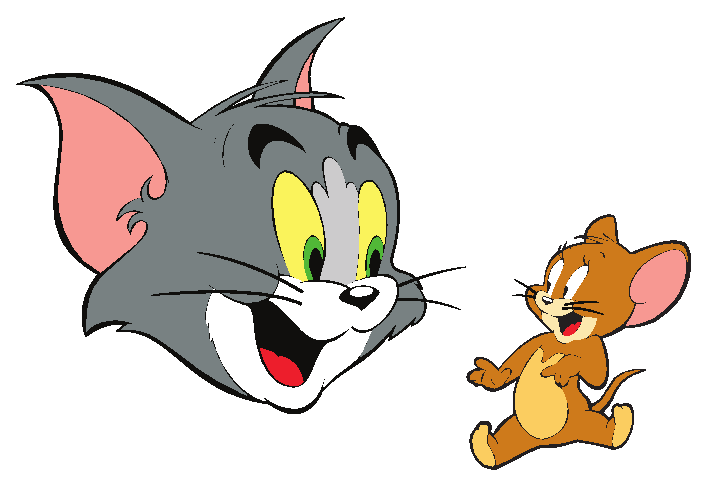
\includegraphics[width=\textwidth]{TomandJerry}
%  \caption{Tom and Jerry}
%    \label{fig:TomJerry}   
%  \end{subfigure}             
%  \begin{subfigure}[b]{0.3\textwidth}
%    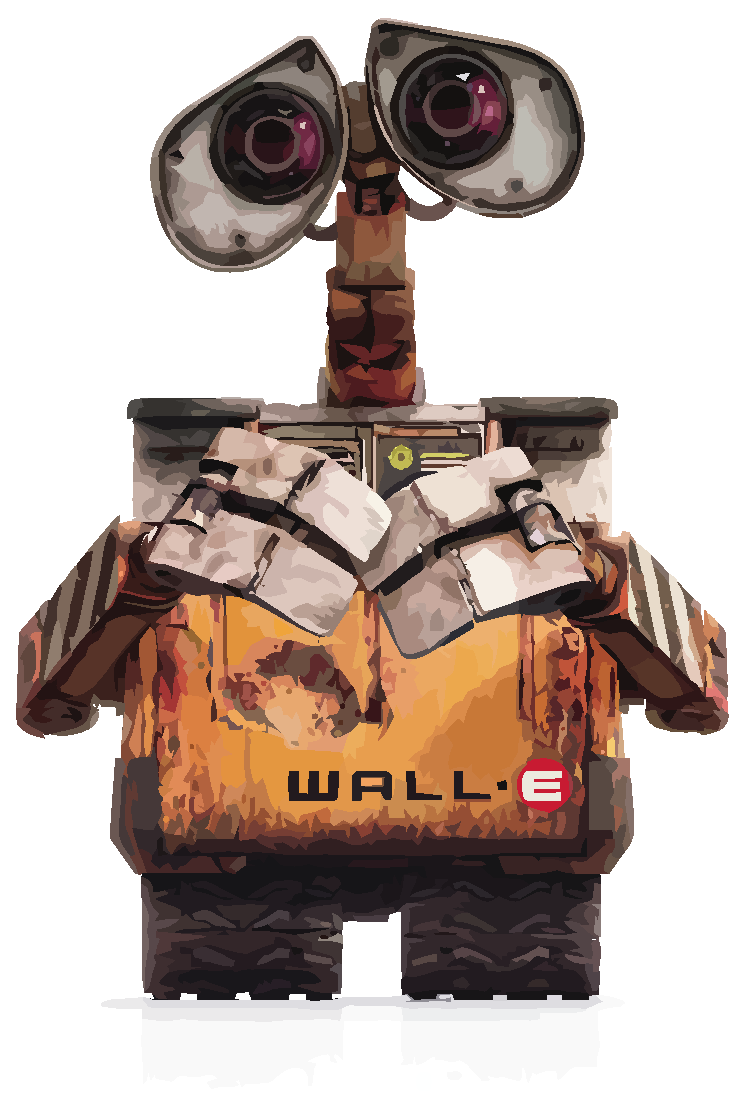
\includegraphics[width=\textwidth]{WallE}
%    \caption{Wall-E}
%    \label{fig:WallE}
%  \end{subfigure}             
%  \begin{subfigure}[b]{0.3\textwidth}
%    
\includegraphics[width=\textwidth]{minion}
%    \caption{Minions}
%    \label{fig:Minnion}
%  \end{subfigure}
%  \caption{Best Animations}
%  \label{fig:animations}
%\end{figure}


